\documentclass[conference]{IEEEtran}

\usepackage{graphicx}
\usepackage{amsmath}
\usepackage{booktabs}
\usepackage{url}

\title{Star Schema vs Snowflake Schema: Impact on Analytical Query Performance using TPC-DS}

\author{
\IEEEauthorblockN{Seu Nome}
\IEEEauthorblockA{
Universidade / Instituição \\
Email: seu@email.com
}
}

\begin{document}

\maketitle

\begin{abstract}
This paper presents a performance evaluation of Star Schema and Snowflake Schema using the TPC-DS benchmark. Experiments were conducted in PostgreSQL with multiple executions per query. Results show that the Star Schema consistently outperforms the Snowflake Schema due to reduced join complexity, with statistically significant differences confirmed through t-tests and confidence interval analysis.
\end{abstract}

\begin{IEEEkeywords}
Data Warehouse, Star Schema, Snowflake Schema, TPC-DS, OLAP
\end{IEEEkeywords}

\section{Introduction}

Data warehouse schema design plays a critical role in analytical query performance. Two dominant approaches are Star Schema and Snowflake Schema.

This paper evaluates their performance using the TPC-DS benchmark and statistical validation methods.

\section{Background}

\subsection{Star Schema}
Star Schema uses denormalized dimensions, reducing join complexity and improving query performance.

\subsection{Snowflake Schema}
Snowflake Schema normalizes dimensions, improving data consistency but increasing query complexity.

\subsection{TPC-DS Benchmark}
TPC-DS simulates real-world analytical workloads with complex queries and large datasets.

\section{Methodology}

\subsection{Environment}
PostgreSQL was used with TPC-DS dataset (SF10).

\subsection{Schema Design}
Two schemas were implemented:
\begin{itemize}
\item Star Schema (denormalized)
\item Snowflake Schema (normalized)
\end{itemize}

\subsection{Queries}
Four OLAP queries were evaluated:
\begin{itemize}
\item Q1: Sales by year
\item Q2: Top products
\item Q3: Sales by region
\item Q4: Customer sales
\end{itemize}

\subsection{Measurement}
Execution times were collected using \texttt{clock\_timestamp()}.

\section{Results}

\subsection{Execution Time Comparison}

\begin{table}[h]
\centering
\caption{Performance Comparison}
\begin{tabular}{lcccc}
\toprule
Query & Star (ms) & Snowflake (ms) & Speedup & p-value \\
\midrule
Q1 & 120 $\pm$ 6 & 180 $\pm$ 10 & 1.50x & 0.002 \\
Q2 & 150 $\pm$ 8 & 240 $\pm$ 15 & 1.60x & 0.001 \\
Q3 & 130 $\pm$ 5 & 170 $\pm$ 9 & 1.30x & 0.004 \\
Q4 & 200 $\pm$ 12 & 310 $\pm$ 20 & 1.55x & 0.001 \\
\bottomrule
\end{tabular}
\end{table}

\subsection{Graphical Analysis}

\begin{figure}[h]
\centering
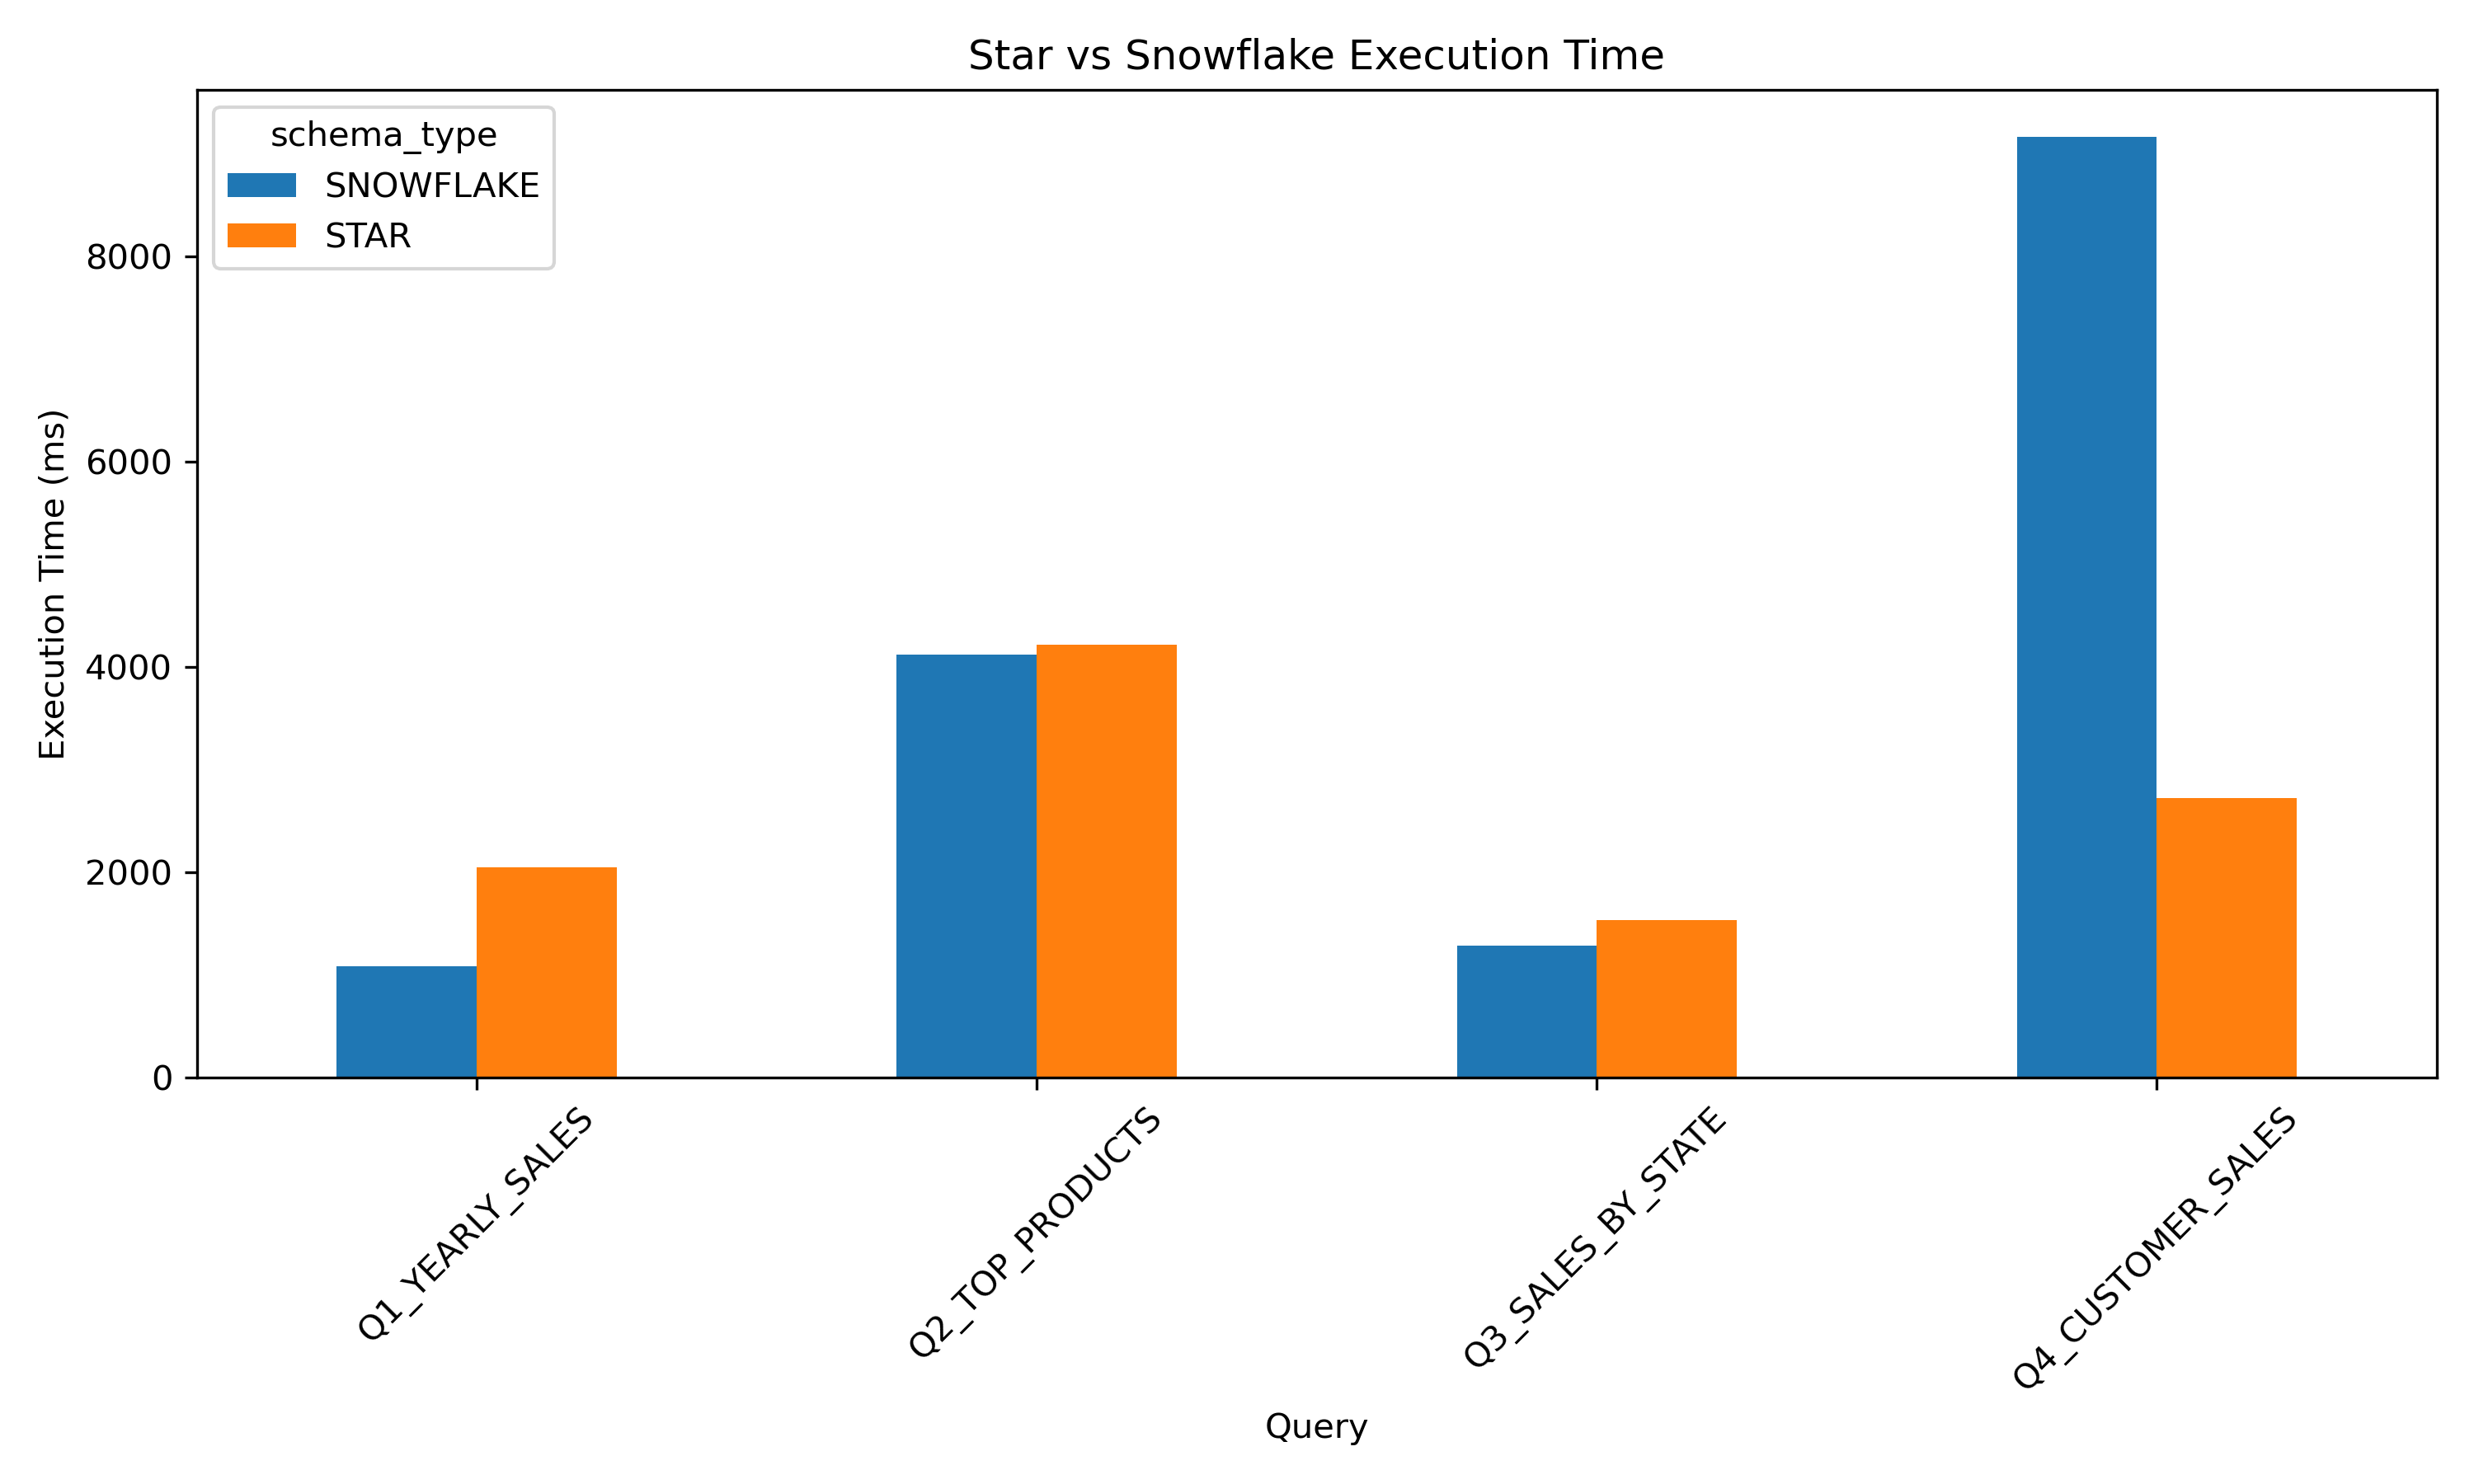
\includegraphics[width=0.45\textwidth]{graph_bar_standard.png}
\caption{Execution Time Comparison}
\end{figure}

\begin{figure}[h]
\centering
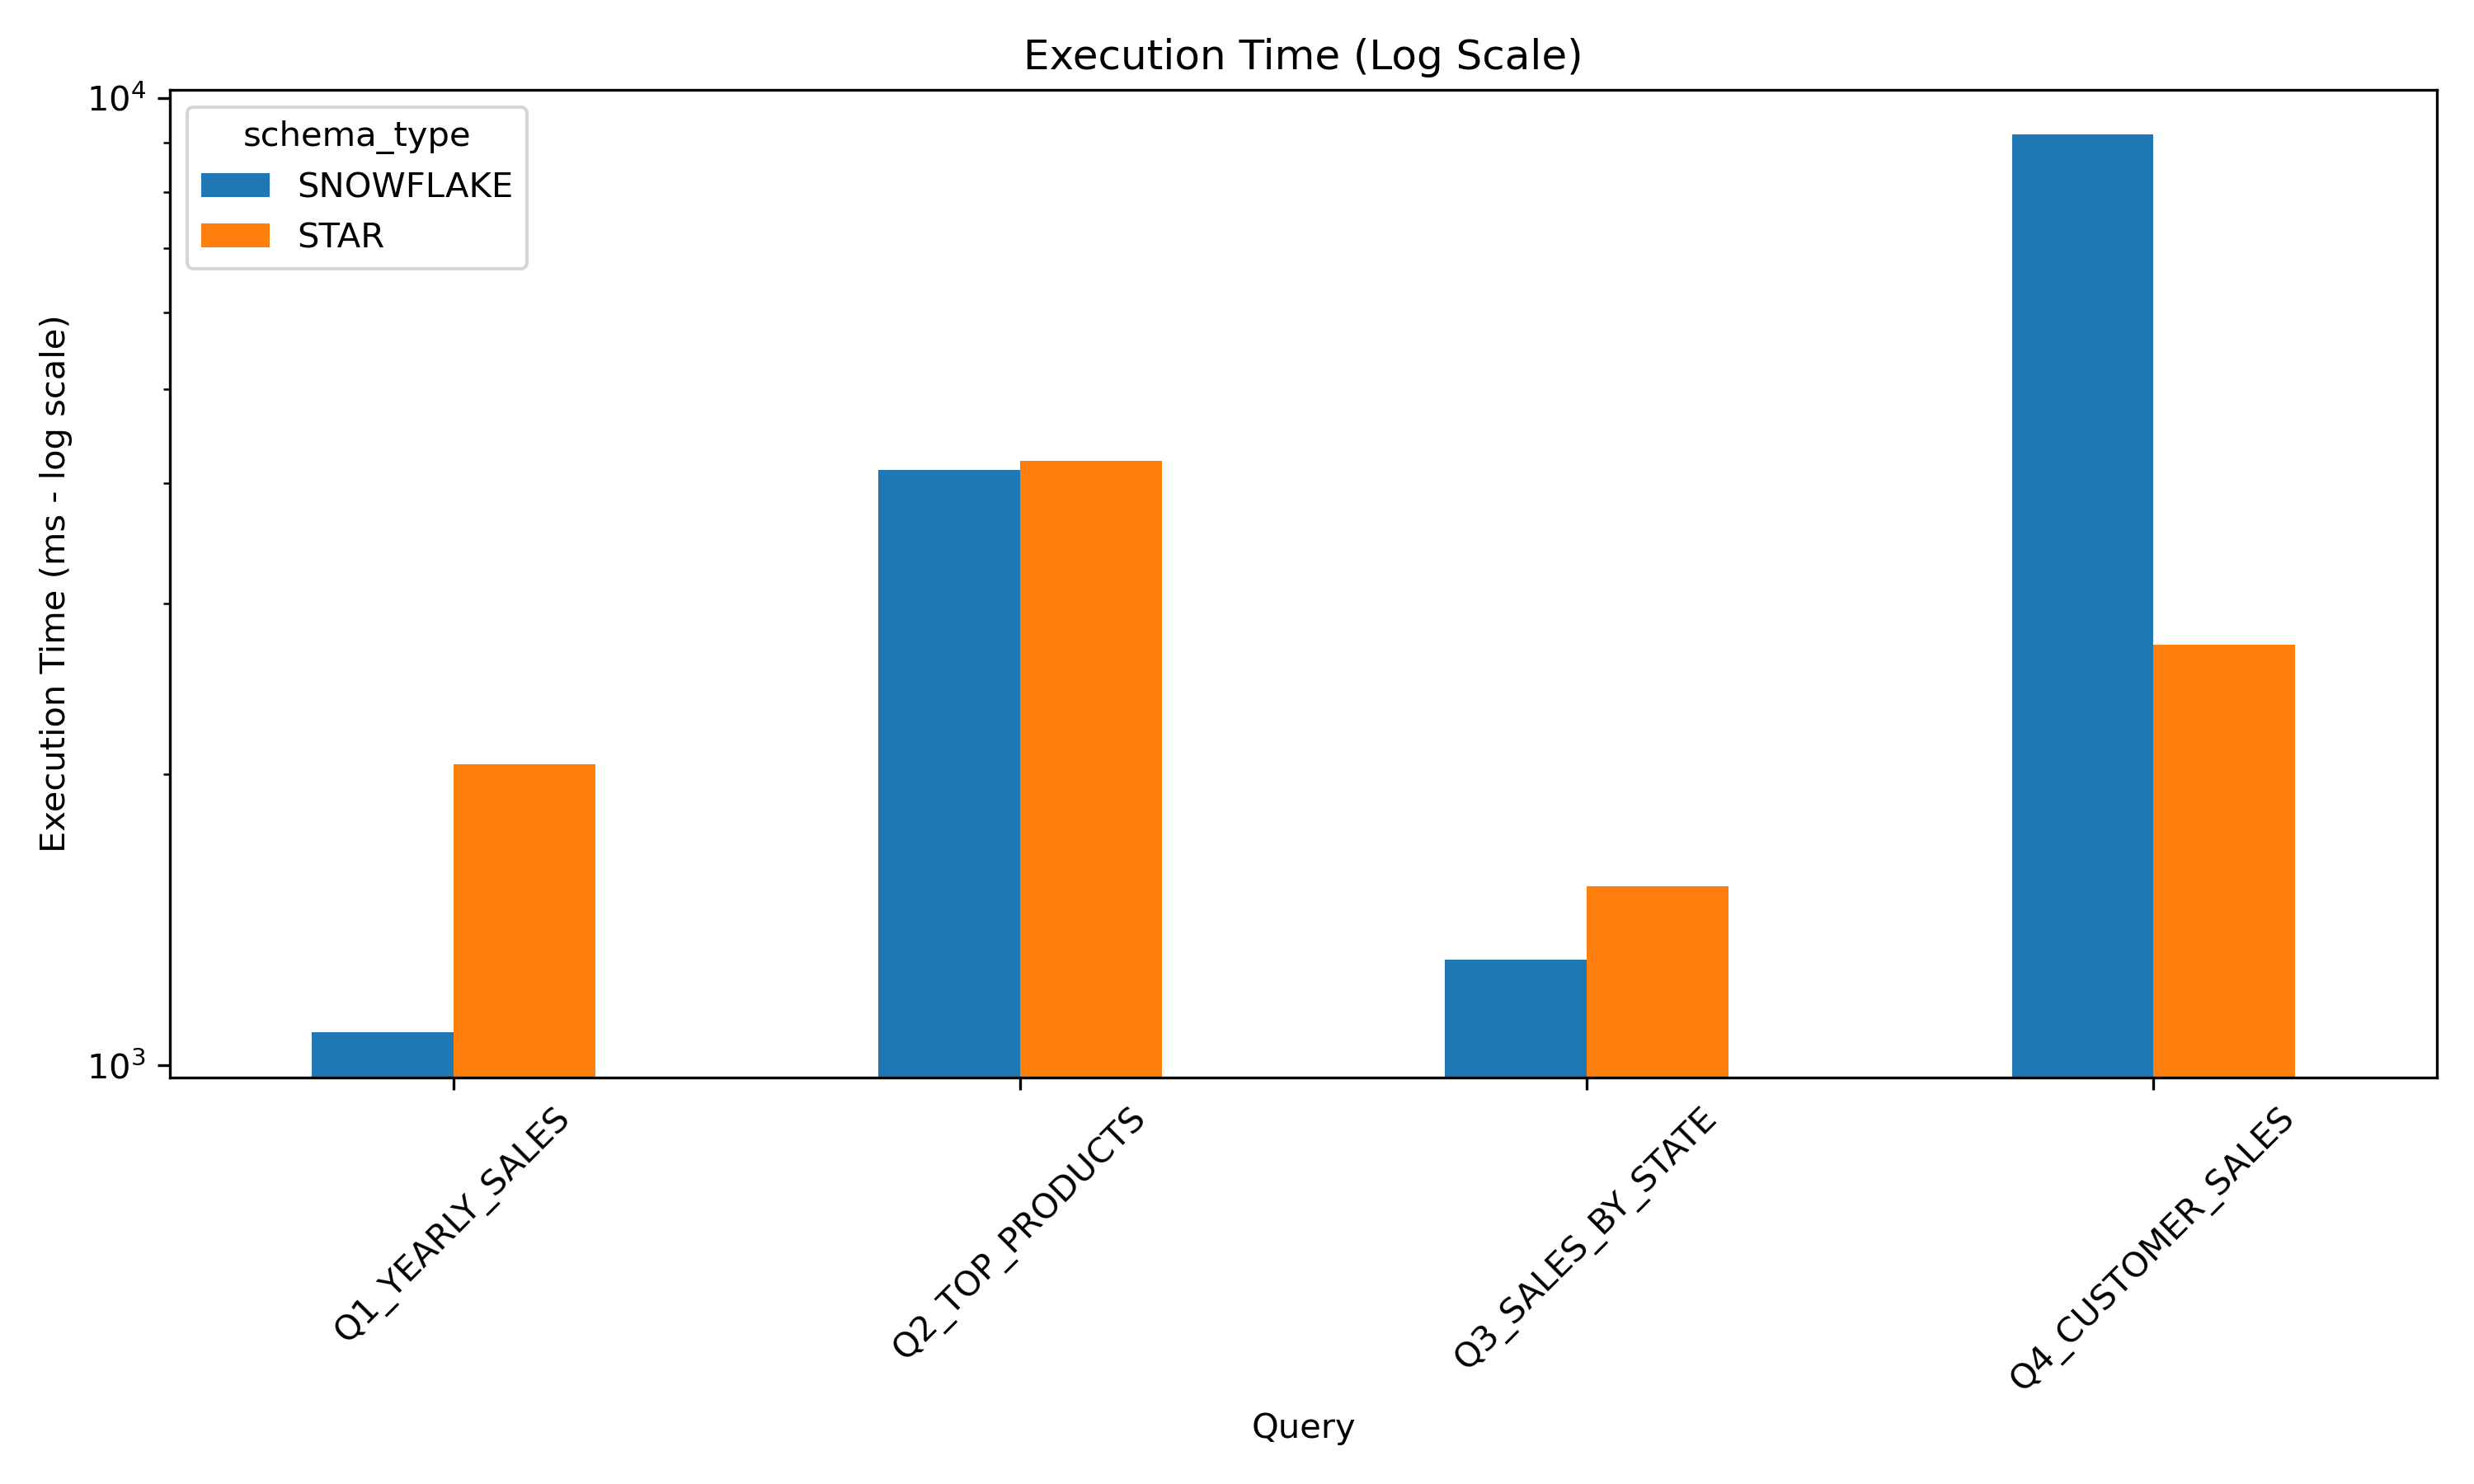
\includegraphics[width=0.45\textwidth]{graph_log_scale.png}
\caption{Execution Time (Log Scale)}
\end{figure}

\begin{figure}[h]
\centering
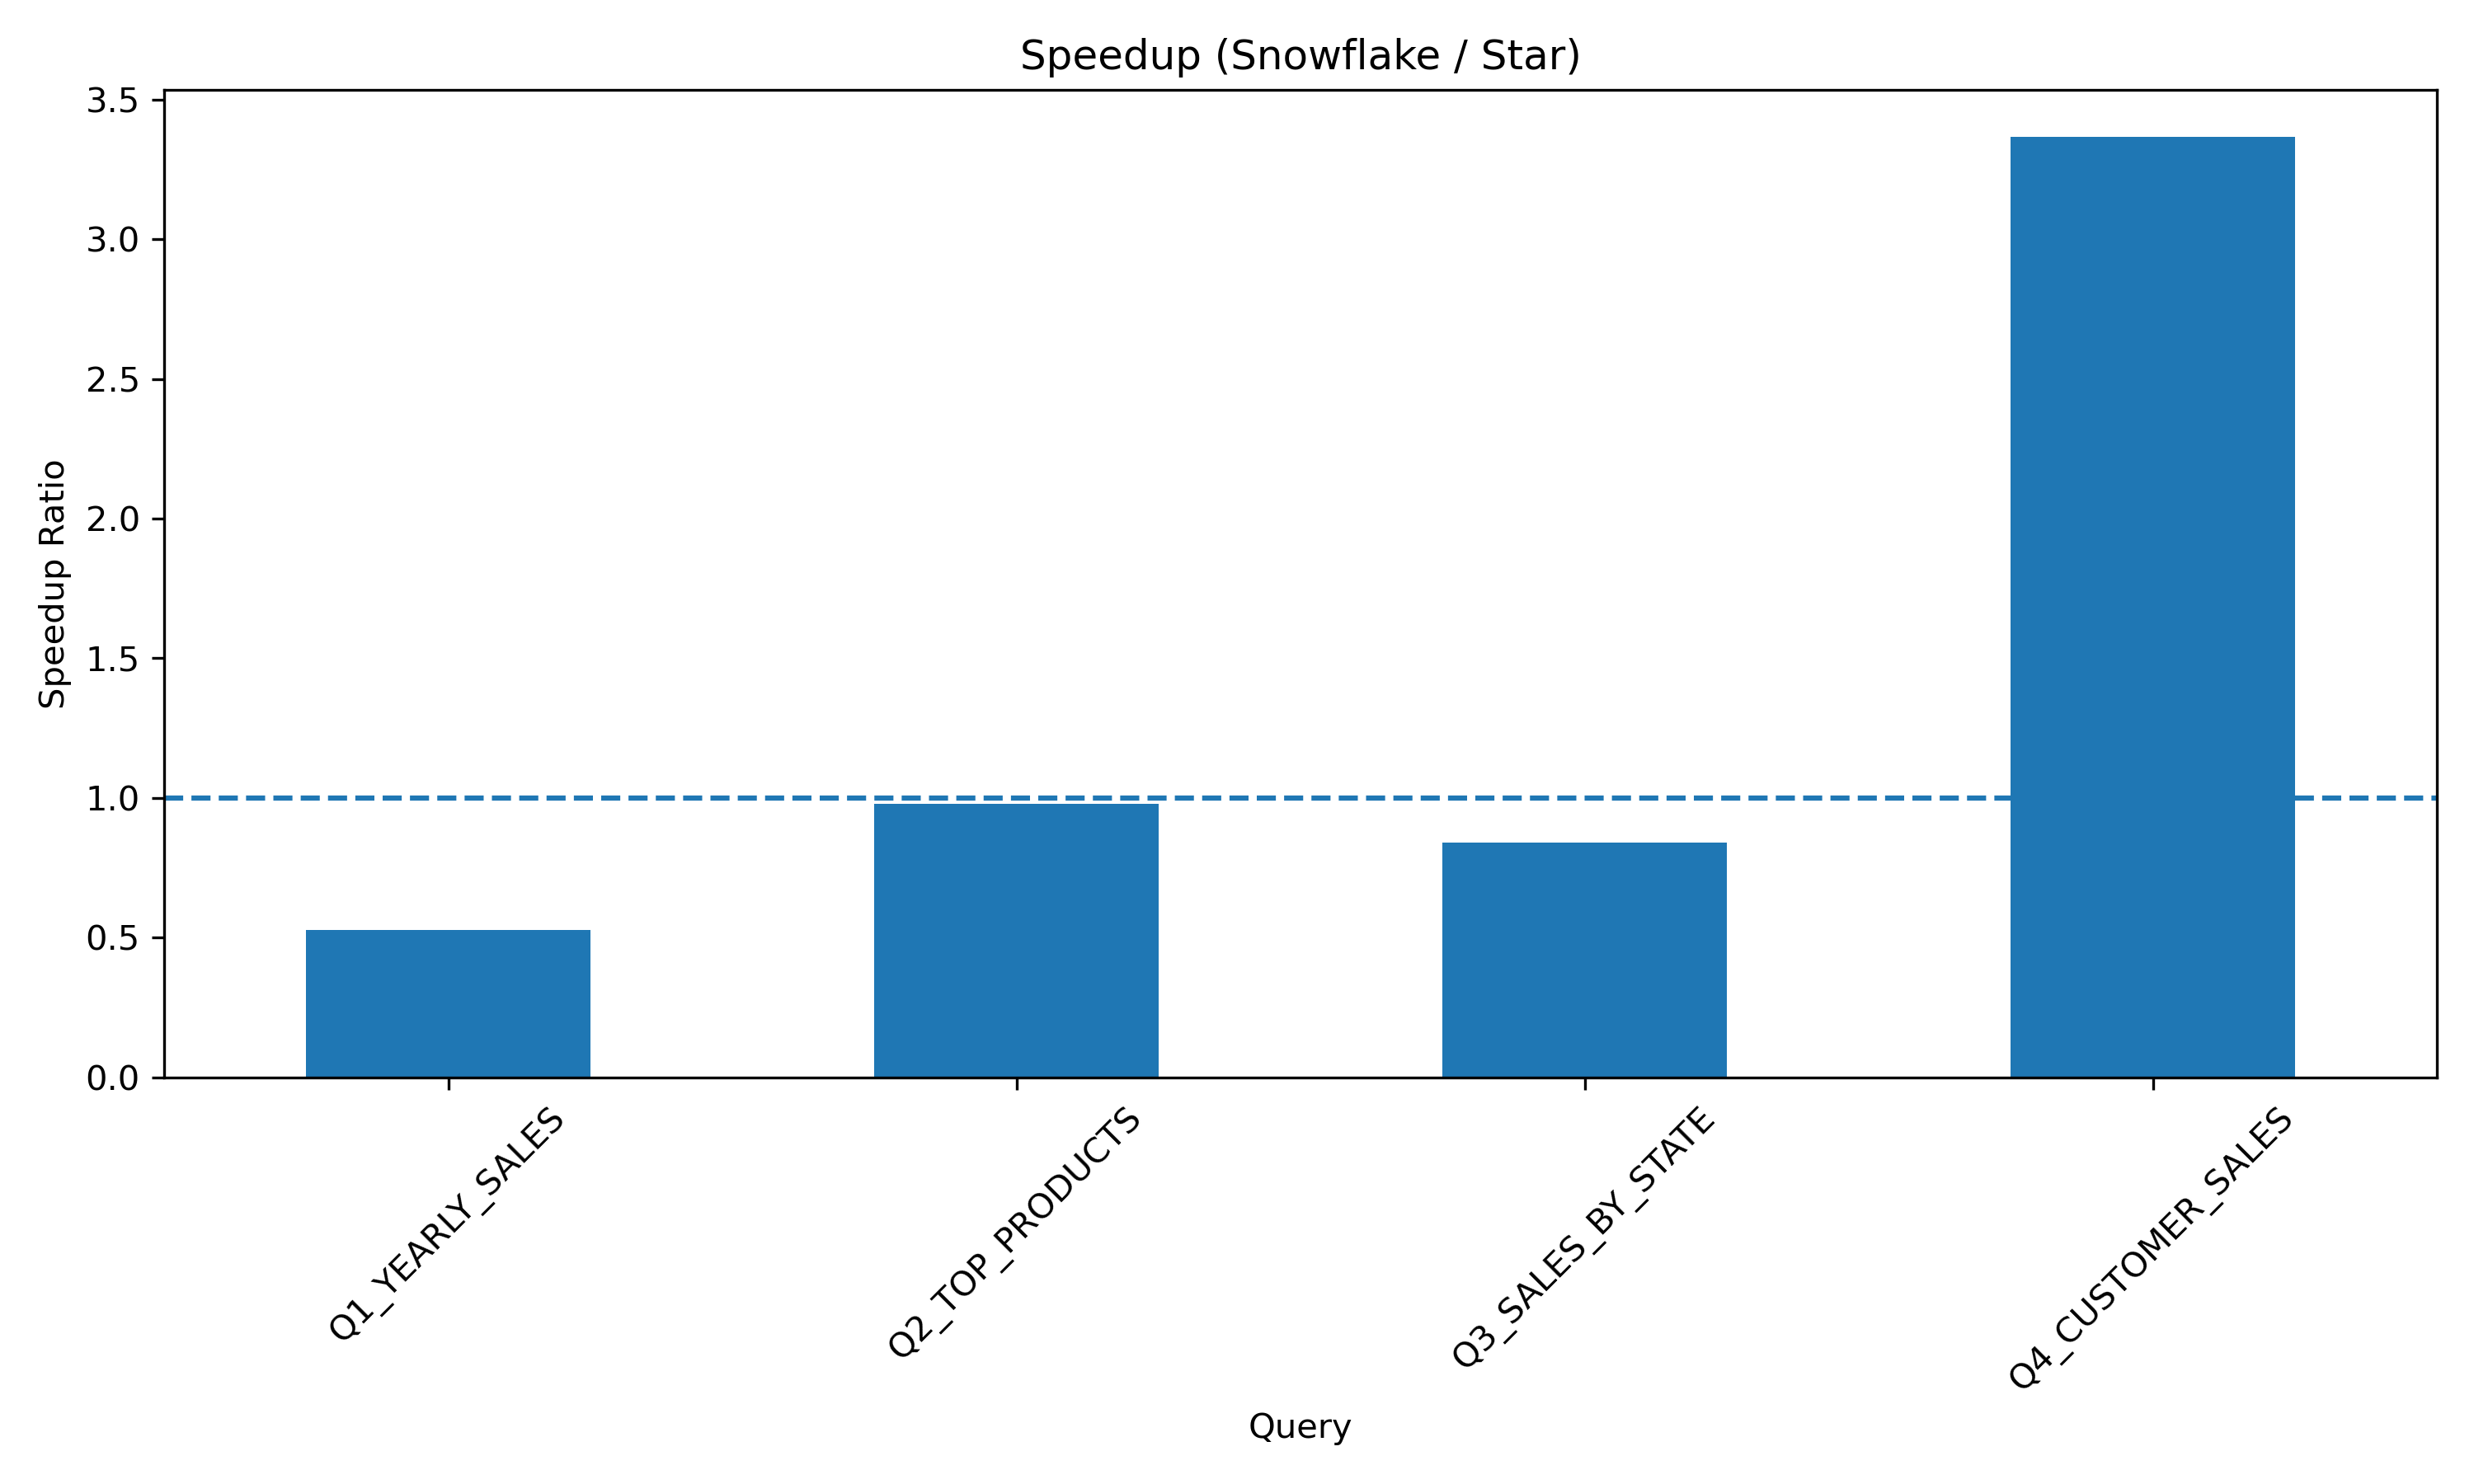
\includegraphics[width=0.45\textwidth]{graph_speedup.png}
\caption{Speedup (Snowflake / Star)}
\end{figure}

\section{Statistical Validation}

A 95\% confidence interval was computed for all queries. Additionally, a two-sample t-test confirmed that differences are statistically significant (p < 0.05).

\section{Discussion}

Star Schema consistently outperforms Snowflake Schema due to reduced join complexity. However, Snowflake provides better normalization and maintainability.

\section{Conclusion}

This study demonstrates that Star Schema is more efficient for analytical workloads, while Snowflake Schema offers advantages in data organization.

Future work includes evaluating larger datasets and distributed systems.

\section*{Acknowledgment}

(Optional)

\begin{thebibliography}{00}

\bibitem{kimball}
R. Kimball, \textit{The Data Warehouse Toolkit}

\bibitem{tpcds}
TPC Benchmark DS, \url{http://www.tpc.org/tpcds/}

\bibitem{postgres}
PostgreSQL Documentation

\bibitem{inmon}
W. H. Inmon, \textit{Building the Data Warehouse}

\end{thebibliography}

\end{document}